\documentclass[10pt]{article}
\usepackage[utf8]{inputenc}
\usepackage[T1]{fontenc}
\usepackage{graphicx}
\usepackage[export]{adjustbox}
\graphicspath{ {./images/} }
\usepackage{amsmath}
\usepackage{amsfonts}
\usepackage{amssymb}
\usepackage[version=4]{mhchem}
\usepackage{stmaryrd}
\usepackage{hyperref}
\hypersetup{colorlinks=true, linkcolor=blue, filecolor=magenta, urlcolor=cyan,}
\urlstyle{same}

\title{CS440: Intro to Artificial Intelligence Assisgnment 1 - 
 Fast Trajectory Replanning }


\author{Adityaraj Gangopadhyay (207001795) and Dharmik Patel (207003436)}
\date{February 25, 2024}


\begin{document}
\maketitle


\section*{Part 0 - Setup your Environments}
We created a depth-first search (DFS) algorithm to generate random mazes of whatever specified size we want. In our maze generation algorithm, we start off with an empty maze, and then starting from a random cell, we mark each cell as visited and decide whether it is blocked or unblocked with a 30\% change of each block being blocked. We select a random neighbor and continue this process. If we reach a 'dead-end, our algorithm backtracks to the last parent node with an un-visited neighbor. This process continues until we have visited every cell. A blocked block is one through which the agent cannot travel through. We also select one random unblocked cell to be the starting (Agent) block and one random unblocked cell to be the target cell.

Below is an example of a randomly generated 101 x 101 size maze. You can also find the A for Agent and T for Target. (You might have to zoom in to see details since the photo is large.):

\begin{center}
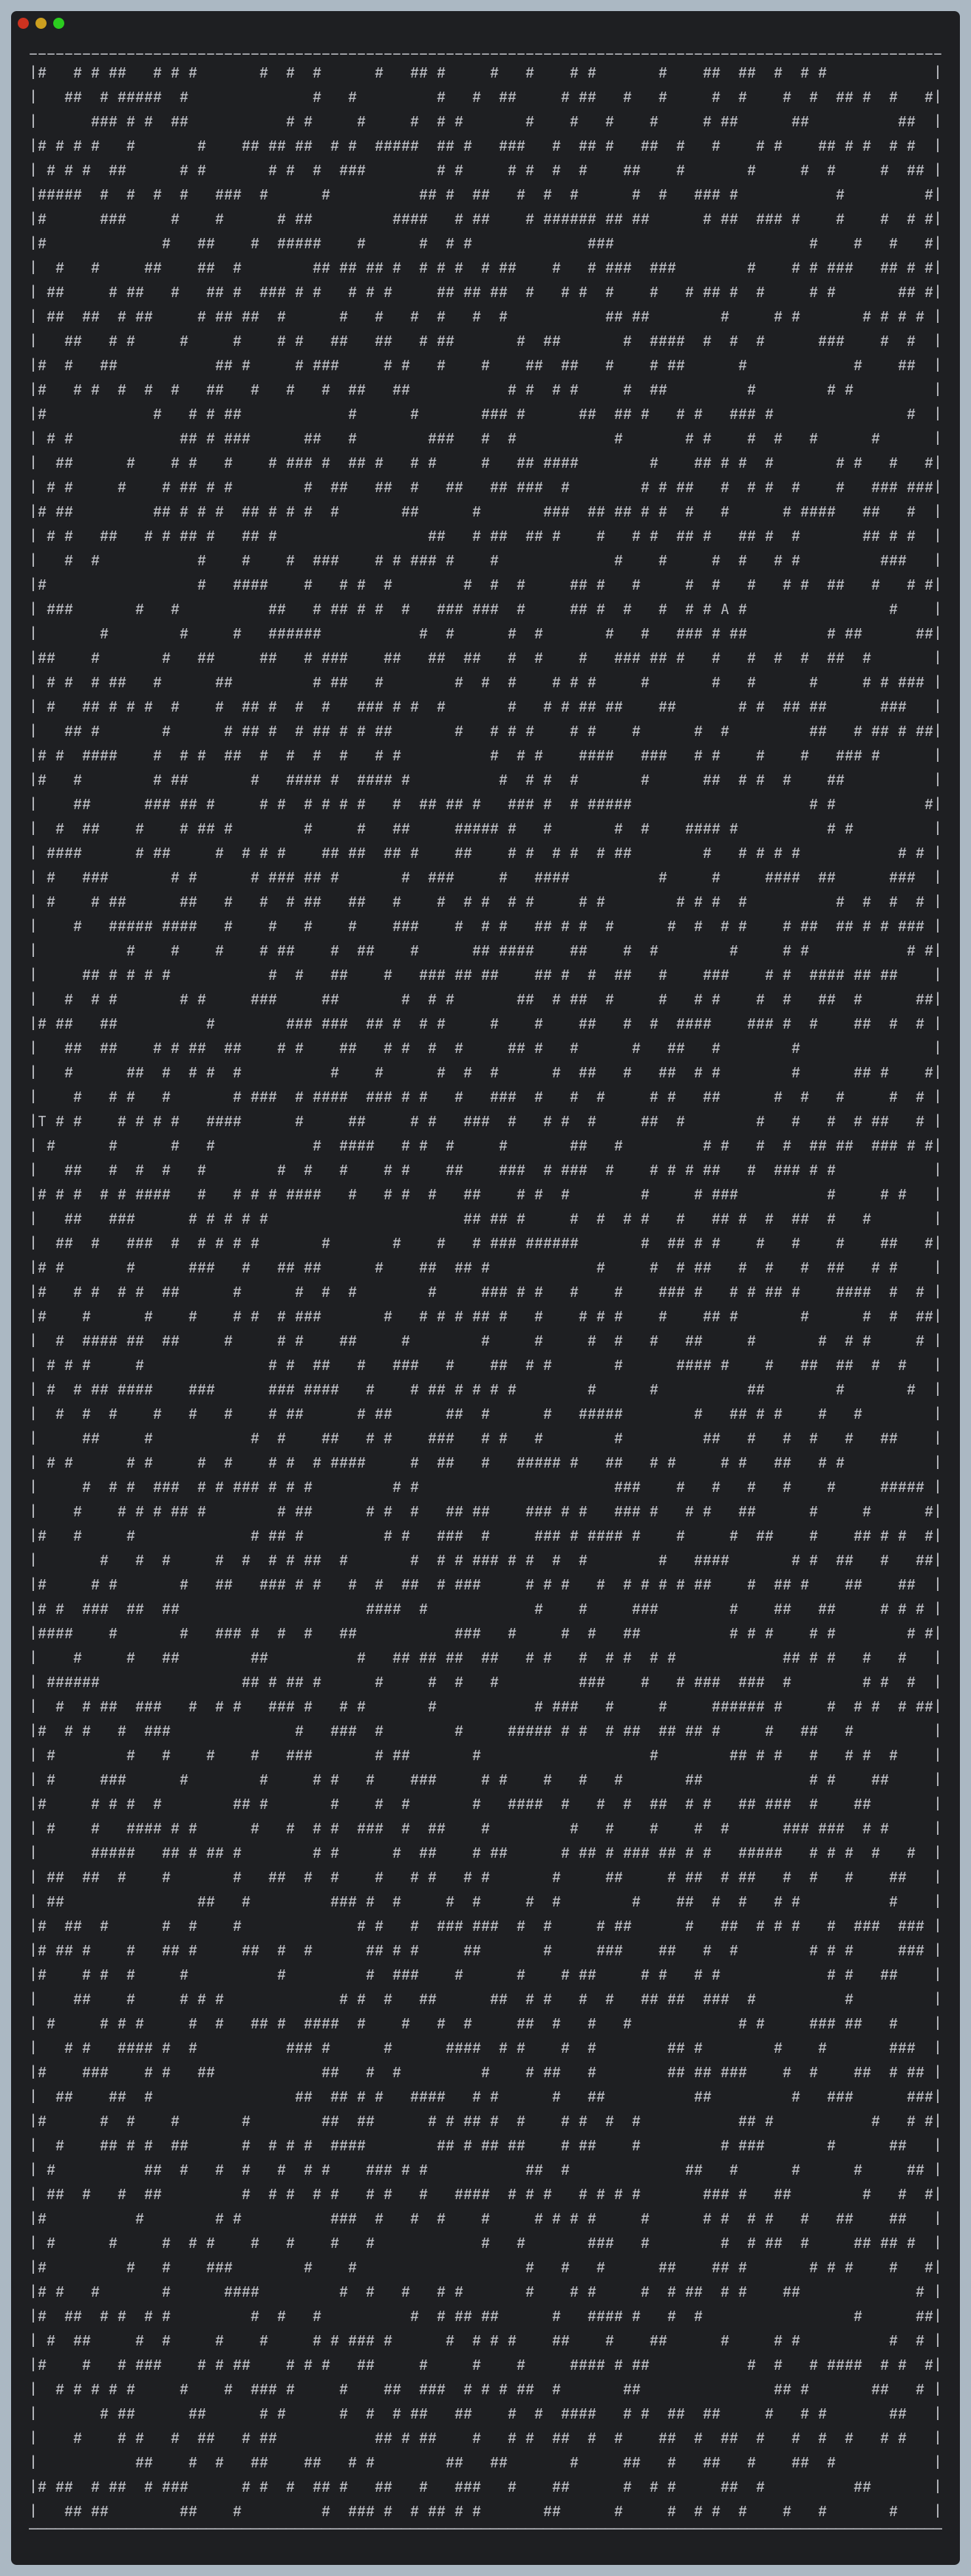
\includegraphics[width=\textwidth,height=\textheight,keepaspectratio]{screenshot.png}
\end{center}

\section*{Part 1 - Understanding the methods}
\begin{center}
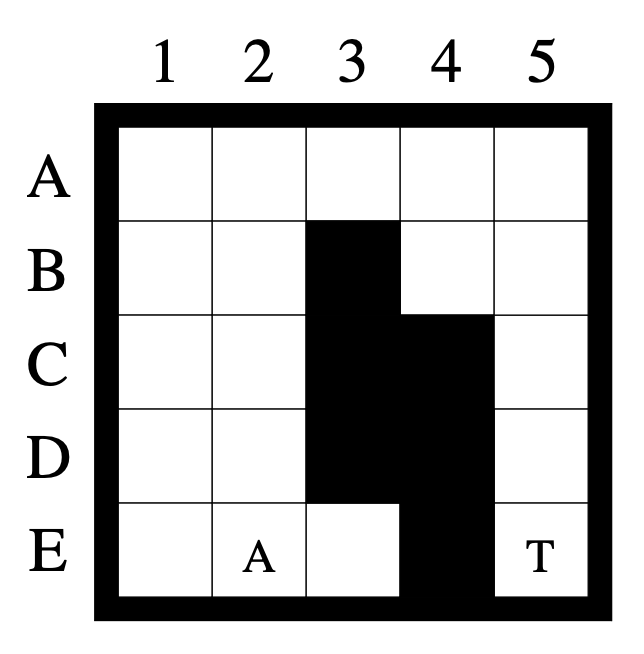
\includegraphics[scale=0.5]{images/E2B94D34-1A9A-49F5-AC00-7BD7A4C3DDC3.png}

\end{center}
a)

The reason why the Agent moved left in the first iteration of A* in Repeated Forward A*, is because at the start, the agent does not know the position of the blocked cells. So the agent calculates the path from $A$ to $T$ as $E2\xrightarrow{}E3\xrightarrow{}E4\xrightarrow{}E5$, because without the blocked cells, that is indeed the fastest path. But, the agent does not see that $E4$ is blocked. Once $E4$ is hit, the agent is re plan the path, but with the updated knowledge of the blocked cells. 

Let us explain this based on $f_{value}$, $g_{value}$, $h_{value}$. The Repeated Forward A will first expanded the start state $A$ and push its 3 neighboring nodes to the open list. The open list is a priority queue which will dequeue the node with the lowest $f_{value}$. 
The 3 neighboring nodes are:
\begin{table}[h!]
\centering
\begin{tabular}{||c c c c ||} 
 \hline
 cell & $f_{value}$ & $g_{value}$ & $h_{value}$ \\ [0.5ex] 
 \hline\hline
E3 & 4 &  1 & 3 \\ 
E1 & 5 & 1 & 4\\ 
D2 & 5 & 1 & 4 \\  
 \hline
\end{tabular}
\caption{ Open List after $E2$ is expanded}
\label{table:0}
\end{table}

The $h_{value}$ are calculated using Manhattan distances, and the $g_{value}$ is the cost of the current path. Since its the first step in a uniform cost maze, the $g_{value}$ is 1.
Therefore, since the agent picks the cell with a lowest $f_{value}$, the agent will pick the first step as $E3$, which is to the left.
\newline
\newline
b)

If the grid world is finite and the agent is not separated by blocked cells from the target, then it can be argued that the agent will either reach the target or discover that it is impossible to do so in finite time. We can prove that the number of moves, until the agent reaches the target or discovers that it is impossible is bounded from above by the number of unblocked cells squared.\newline

 We can prove this because, in the worst-case scenario, the agent would need to traverse each cell once to discover and once to backtrack to it. The number of unblocked cells is finite. Therefore, the amount of time required is finite, and the number of moves is bounded by the number of unblocked cells squared. 

We can demonstrate this with the following equation:
\newline
\newline
$m \le u^{2}$
\newline
\newline

Where $m$ is the number of moves made, and $u$ is the number of unblocked cells. If our grid is finite, our $u$ is finite, and $m$ is less than or equal to $u^{2}$.


\section*{Part 2 - The Effects of Ties}
\begin{table}[h!]
\centering
\begin{tabular}{||c c c ||} 
 \hline
 Algorithm & Favor Higher G Value & Favor Lower G Value \\ [0.5ex] 
 \hline\hline
 Repeated Forwards & 14.6 & 157.74 \\ 
 Repeated Backwards & 13.28 & 169.68 \\ 
 Repeated Adaptive & 14.22 &  153.82 \\ 
 \hline
\end{tabular}
\caption{Average Runtime(ms) on 50 Random Mazes}
\label{table:1}
\end{table}
\begin{table}[h!]
\centering
\begin{tabular}{||c c c ||} 
 \hline
 Algorithm & Favor Higher G Value & Favor Lower G Value \\ [0.5ex] 
 \hline\hline
 Repeated Forwards & 2098 & 29873 \\ 
 Repeated Backwards & 1920 & 31814 \\ 
 Repeated Adaptive & 2069 &  29400 \\ 
 \hline
\end{tabular}
\caption{ Average Number of Nodes Expanded on 50 Random Mazes.}
\label{table:2}
\end{table}


\textbf{Implementation:} Our node object overrides the dunder method ${lt()}$. In the dunder method, it will first compare the $f_{values}$. If the $f_{values}$ are equal, then we have entered tie breaking. If we want to favor larger $g_{values}$, we would return the node with the higher $g_{values}$, and if we want to favor lower $g_{values}$, then we would return the node with the lower $g_{values}$. 

\textbf{Observations and Reasoning:} In all 3 versions of A*, when we favor higher $g_{values}$, the agent will find the goal about 10x faster. See table 1 and 2. To understand how one simple change can have such a massive effect, we must know what the $g_{values}$ represent. The $g_{values}$ are the current incurred cost. When we say "favoring a node", we will dequeue it from open list priority queue earlier. If we favor lower $g_{values}$, then we will pop nodes that are closer to the start state before nodes that are further away. That means the agent will explore all the nodes closer to the start before exploring closer to the goal. But when you favor higher $g_{values}$, we let the agent explore more towards the goal, without the need to explore closer to the start. Since the agent is able to explore closer to the goal, the agent finds the goal faster when we favor higher $g_{values}$.

\section*{Part 3 - Forward vs. Backward}

\textbf{Implementation:} Once we have forward A* implemented, we just swap the start and goals states in backwards A*. \textbf{Observations and Reasoning:}
In some maze runs, backwards A* expands less nodes, and in some maze runs, forwards A* expands less nodes. See table 1 and 2. It is based on how "crowded" the maze is at either end. If the maze is more "crowded" then that means there are more dead ends. The location of the dead ends matter because of the inherit direction of the algorithm. Therefore, there is no advantage in using Forwards or Backwards over each other, if the actual maze is symmetrical. But the asymmetric nature of the maze, might cause in some cases for Forward A* to beat Backwards A*, or vice versa. So the difference in performance is due to the maze layout it self. 




\section*{Part 4 - Heuristics in the Adaptive A*}

\textbf{Proof of Manhattan Distance being consistent}
Manhattan Distance: \(h(n) = |n_x - g_x|+|n_y - g_y|\) where g = goal state

The definition of an heuristic function \(h(n)\) being consistent is \[\forall(n, a, n'):\;\;\;h(x) \le c(n, a, n') + h(n') \;\;\; and \;\;\; h(n) = 0 \;\;\; if \;\;\; n = goal\]
Proof for when \(n = goal = g\): 
\begin{gather*} 
h(n) = |n_x - g_x|+|n_y - g_y| \\ 
h(g) = |g_x - g_x|+|g_y - g_y| \\
h(g) = |0|+|0| \\
h(g) = 0
\end{gather*}
Proof for when \(n \ne goal\):
We can prove that the Manhattan distance is consistent by using the triangle inequality: where if you have 3 sides of a triangle, lengths a, k and c, then \(c \le k +b\). If we let
\begin{gather*} 
k = c(n, a, n') \\
b = h(n') \\
c = h(n) \\
\end{gather*}
and more specify, point \(n, n', goal\) are the corners of a triangle, \(h(n)\) is the distance from \(n\) to \(goal\), \(h(n')\) is the distance from \(n'\) to \(goal\), and \(c(n, a, n')\) is the step cost from \(n\) to \(n'\).  

So using the triangle inequality, and substituting the values for \(c, k, b\) from above:
\begin{gather*} 
c \le k + b \\ 
h(n) \le c(n, a, n') + h(n')
\end{gather*}
we prove that $h(n)$ fits the definition of consistency.

\textbf{Prove that Adaptive A* leaves initially consistent h-values consistent even if action costs can increase.}From above, we have proved that the Manhattan distance is consistent:
\[h(n) \le c(n, a, n') + h(n')\]
In Adaptive A*, the can action cost increases. So let \(c'\) denote the new increases action cost. 
\[c(n, a, n') \le c'(n, a, n')\]
If we substitute \(c'\) in for \(c\):
\begin{gather*} 
h(n) \le c(n, a, n') + h(n') \\ 
h(n) \le c'(n, a, n') + h(n')
\end{gather*}
the inequality still holds true. Therefore with the new increase action cost, our heuristic function still matches the definition of consistency.

\section*{Part 5 - Repeated Forward A* vs Adaptive A*}
\textbf{Implementation: }We used a global dict to hold $h_{values}$ and have them persist through multiple re-plannings. \textbf{Observations and Reasoning: }On average, Adaptive A* will run faster and expand fewer nodes compared to Repeated Forwards A* (Table 1 and 2). This is due to Adaptive A* recalculating the $h_{values}$. The recalculation will better guide the agent towards the goal, and avoid expanding unnecessary nodes. Also the new heuristic function dominates the Manhattan distance, and thus is a better estimate of the real cost.

\section*{Part 6 - Statistical Significance}

It is true that performance differences between two search algorithms can be either systematic in nature or only due to sampling noise. One can use statistical hypothesis tests to determine whether  they truly are systematic in nature.\newline

If we were to take Part 5, where we compare Repeated Forward A* with Adaptive A*, and were to perform a statistical hypothesis test to determine if Adaptive A* is significantly faster than Repeated Forward A*, we would start off with establishing a Null Hypothesis and an Alternative Hypothesis. The Null hypothesis would state that there is no significant difference in speed between the algorithms and the alternative hypothesis would state there is a significant difference in speed between the algorithms. We then choose and perform a statistical test. In this case, that would run repeated forward A* and adaptive A* multiple times on the different mazes. We collect the means and standard deviations of runtime for both algorithms. From this, we calculate the test statistic. We then determine the significance level and calculate the p-value. We can also determine the critical value. We then decide whether we reject or fail to reject the null hypothesis. If the test statistic is lower than the critical value or if the p-value is less than the significance level we reject the null hypothesis, otherwise we do not. If we reject the null hypothesis, then we are claiming that there is a significant difference in the speed of the algorithms.

\section*{References}

Hosch, William L.. "triangle inequality". \textit{Encyclopedia Britannica,} 3 Jan. 2024, https://www.britannica.com/science/triangle-inequality. Accessed 26 February 2024.\newline


\noindent Hayes, A. (2022, July 20). T-Test: What It Is With Multiple Formulas and When To Use Them. Retrieved from Investopedia website: https://www.investopedia.com/terms/t/t-test.asp

 
\end{document}